 
\chapter{Logistic Regressions for Categorical Outcomes} 
  \chaptermark{Multinomial and Proportional Odds Model}
\label{chapter::logit-categorical}
 

Categorical outcomes are common in empirical research. The first type of categorical outcome is nominal. For example, the outcome denotes the preference for fruits (apple, orange, and pear) or transportation services (Uber, Lyft, or BART). The second type of categorical outcome is ordinal. For example, the outcome denotes the course evaluation at Berkeley (1, 2, \ldots, 7) or Amazon review (1 to 5 stars).  
This chapter discusses statistical modeling strategies for categorical outcomes, including two classes of models corresponding to the nominal and ordinal outcomes, respectively.  
 
 

\section{Multinomial distribution}



A categorical random variable $y$ taking values in $\left\{ 1,\ldots,K\right\} $
with probabilities $\pr(y=k)=\pi_{k}$  ($k=1,\ldots,K$) is
often called a multinomial distribution, denoted by
\begin{equation}
y\sim\text{Multinomial}\left\{ 1;(\pi_{1},\ldots,\pi_{K})\right\} ,\label{eq:multinomial-rv}
\end{equation}
where $\sum_{k=1}^{K}\pi_{k}=1.$
We can calculate the mean and covariance matrix of $y$:
\begin{proposition}
\label{proposition:positive-semi-definite-multinomial}If $y$ is the Multinomial
random variable in (\ref{eq:multinomial-rv}), then $(1(y=1),\ldots,1(y=K-1))$
has mean $(\pi_{1},\ldots,\pi_{K-1})$ and covariance matrix
\begin{equation}
\left(\begin{array}{cccc}
\pi_{1}(1-\pi_{1}) & -\pi_{1}\pi_{2} & \cdots & -\pi_{1}\pi_{K-1}\\
-\pi_{1}\pi_{2} & \pi_{2}(1-\pi_{2}) & \cdots & -\pi_{2}\pi_{K-1}\\
\vdots & \vdots & \ddots & \vdots\\
-\pi_{1}\pi_{K-1} & -\pi_{2}\pi_{K-1} & \cdots & \pi_{K-1}(1-\pi_{K-1})
\end{array}\right).\label{eq:cov-multinomial-rv}
\end{equation}
As a byproduct, we know that the matrix in (\ref{eq:cov-multinomial-rv})
is positive semi-definite.
\end{proposition}



\begin{myproof}{Proposition}{\ref{proposition:positive-semi-definite-multinomial}}
Without loss of generality, I will calculate the $(1,1)$th and the $(1,2)$th element of the matrix. First, $1(y=1)$ is Bernoulli with probability $\pi_1$, so the $(1,1)$th element equals var$( 1(y=1) ) = \pi_1 (1 - \pi_1)$. Similarly, the $(2,2)$th element equals var$( 1(y=2) ) = \pi_2 (1 - \pi_2)$.

Second, $1(y=1) +1(y=2)$ is Bernoulli with probability $\pi_1 + \pi_2$, so var$(1(y=1) +1(y=2)) = (\pi_1 + \pi_2)(1-\pi_1 -\pi_2)$. Therefore, the $(1,2)$-th element equals
\begin{eqnarray*}
&&\cov(1(y=1), 1(y=2) ) \\
&=& \left\{ \var( 1(y=1) +1(y=2) ) - \var( 1(y=1)) - \var(1(y=2)) \right\} / 2 \\
&=& -\pi_1 \pi_2.
\end{eqnarray*}  
\end{myproof}



With independent samples of $(x_{i},y_{i})_{i=1}^{n}$, we want to
model $y_{i}$ based on covariates $x_{i}$\footnote{An alternative  strategy is to model $1(y_i=k)\mid x_i$ for each $k$. The advantage of this strategy is that it reduces to binary logistic models. The disadvantage of this strategy is that it does not model the whole distribution of $y_i$ and can lose efficiency in estimation.}:
\[
y_{i}\mid x_{i}\sim\text{Multinomial}\left[1;\left\{ \pi_{1}(x_{i}),\ldots,\pi_{K}(x_{i})\right\} \right],
\]
where $\sum_{k=1}^{K}\pi_{k}(x_{i})=1$  for all $x_{i}.$
We can write the probability mass function of $\pr( y_{i}\mid x_{i} ) $ as
\begin{eqnarray*}
\pi_{y_i}(x_i) 
&=& 
  \prod_{k=1}^{K}  \left\{   \pi_{k}(x_{i}) \text{ if } y_{i}=k\right\}  \\
&=&  \prod_{k=1}^{K}\left\{ \pi_{k}(x_{i})\right\} ^{1(y_{i}=k) }.
\end{eqnarray*}
Here $\pi_{k}(x_{i} ) $ is a general function of $x_i$. The remaining parts of this chapter will discuss the canonical choices of $\pi_{k}(x_{i} ) $ for nominal and ordinal outcomes. 




\section{Multinomial logistic model for nominal outcomes}

\subsection{Modeling}
Viewing category $K$ as the reference level, we can model the ratio of
the probabilities of categories $k$ and $K$ as
\[
\log\frac{\pi_{k}(x_{i})}{\pi_{K}(x_{i})}=x_{i}^{\T}\beta_{k}\qquad(k=1,\ldots,K-1)
\]
which implies that 
\[
\pi_{k}(x_{i})=\pi_{K}(x_{i})e^{x_{i}^{\T}\beta_{k}}\qquad(k=1,\ldots,K-1).
\]
Due to the normalization, we have
\[
\begin{array}{cclr}
\sum_{k=1}^{K}\pi_{k}(x_{i})=1 & \Longrightarrow& \sum_{k=1}^{K}\pi_{K}(x_{i})e^{x_{i}^{\T}\beta_{k}}=1\\
 & \Longrightarrow&\pi_{K}(x_{i})\sum_{k=1}^{K}e^{x_{i}^{\T}\beta_{k}}=1\\
 & \Longrightarrow&\pi_{K}(x_{i})=1\Big/\sum_{k=1}^{K}e^{x_{i}^{\T}\beta_{k}}\\
 & \Longrightarrow&\pi_{k}(x_{i})=\frac{e^{x_{i}^{\T}\beta_{k}}}{\sum_{ l =1}^{K}e^{x_{i}^{\T}\beta_{ l }}} & (k=1,\ldots,K-1).
\end{array}
\]
A more compact form is 
\begin{eqnarray}
\pi_{k}(x_{i})=\pi_{k}(x_{i},\beta)=\frac{e^{x_{i}^{\T}\beta_{k}}}{\sum_{ l =1}^{K}e^{x_{i}^{\T}\beta_{ l }}},\qquad(k=1,\ldots,K)
\label{eq::multinomial-logistic}
\end{eqnarray}
where $\beta=(\beta_{1},\ldots,\beta_{K-1})$ denotes the parameter
with $\beta_{K}=0$ for the reference category. From the ratio form of \eqref{eq::multinomial-logistic}, we can only identify $\beta_k - \beta_K$ for all $k= 1,\ldots, K$. So for convenience, we impose the restriction $\beta_{K}=0$. 
Model \eqref{eq::multinomial-logistic} is called the multinomial logistic regression model. 


Similar to the binary logistic regression model, we can interpret the coefficients as the conditional log odds ratio compared to the reference level:
\begin{align*}
\beta_{k,j} & =\log\frac{\pi_{k}( \ldots,x_{ij}+1,\ldots )}{\pi_{K}( \ldots,x_{ij}+1,\ldots )}-\log\frac{\pi_{k}( \ldots,x_{ij},\ldots )}{\pi_{K}( \ldots,x_{ij},\ldots )}\\
 & =\log\left\{ \frac{\pi_{k}( \ldots,x_{ij}+1,\ldots )}{\pi_{K}( \ldots,x_{ij}+1,\ldots )}\Big/\frac{\pi_{k}( \ldots,x_{ij},\ldots )}{\pi_{K}( \ldots,x_{ij},\ldots )}\right\} .
\end{align*}


\subsection{MLE}
The likelihood function for the multinomial logistic model is
\begin{align*}
L(\beta) & =\prod_{i=1}^{n}\prod_{k=1}^{K}\left\{ \pi_{k}(x_{i})\right\} ^{1(y_{i}=k)}\\
 & =\prod_{i=1}^{n}\prod_{k=1}^{K}\left\{ \frac{e^{x_{i}^{\T}\beta_{k}}}{\sum_{ l =1}^{K}e^{x_{i}^{\T}\beta_{ l }}}\right\} ^{1(y_{i}=k)}\\
 & =\prod_{i=1}^{n}
\left[  
 \left\{ \prod_{k=1}^{K}e^{1(y_{i}=k)x_{i}^{\T}\beta_{k}}\right\}  \Big/\sum_{k=1}^{K}e^{x_{i}^{\T}\beta_{k}}
 \right],
\end{align*}
and
the log-likelihood function is
\[
\log L(\beta)=\sumn
\left[ 
\sum_{k=1}^{K} 1(y_{i}=k)x_{i}^{\T}\beta_{k}-\log\left\{ \sum_{k=1}^{K}e^{x_{i}^{\T}\beta_{k}}\right\} \right].
\]
The score function is 
$$
\frac{\partial\log L(\beta)}{\partial\beta} = \begin{pmatrix}
\frac{\partial\log L(\beta)}{\partial\beta_{1}}\\
\vdots\\
\frac{\partial\log L(\beta)}{\partial\beta_{K-1}} 
\end{pmatrix}
\in \mathbb{R}^{p(K-1)}
$$
with 
\begin{align*}
\frac{\partial\log L(\beta)}{\partial\beta_{k}} & =\sumn\left\{ x_{i}1(y_{i}=k)-\frac{x_{i}e^{x_{i}^{\T}\beta_{k}}}{\sum_{ l =1}^{K}e^{x_{i}^{\T}\beta_{ l }}}\right\} \\
 & =\sumn x_{i}\left\{ 1(y_{i}=k)-\frac{e^{x_{i}^{\T}\beta_{k}}}{\sum_{ l =1}^{K}e^{x_{i}^{\T}\beta_{ l }}}\right\} \\
 & =\sumn x_{i}\left\{ 1(y_{i}=k)-\pi_{k}(x_{i},\beta)\right\}  \in \mathbb{R}^{p}  ,\quad(k=1,\ldots,K-1).
\end{align*}
The Hessian matrix is 
\begin{eqnarray}
\frac{\partial^{2}\log L(\beta)}{\partial\beta \partial\beta^{\T}}
=\begin{pmatrix}
\frac{\partial^{2}\log L(\beta)}{\partial\beta_{1}\partial\beta_{1}^{\T}}  & \frac{\partial^{2}\log L(\beta)}{\partial\beta_{1}\partial\beta_{2}^{\T}}  & \cdots & \frac{\partial^{2}\log L(\beta)}{\partial\beta_{1}\partial\beta_{K-1}^{\T}}  \\
\frac{\partial^{2}\log L(\beta)}{\partial\beta_{2}\partial\beta_{1}^{\T}}  & \frac{\partial^{2}\log L(\beta)}{\partial\beta_{2}\partial\beta_{2}^{\T}}  & \cdots & \frac{\partial^{2}\log L(\beta)}{\partial\beta_{2}\partial\beta_{K-1}^{\T}}  \\
\vdots &\vdots  &&\vdots \\
\frac{\partial^{2}\log L(\beta)}{\partial\beta_{K-1}\partial\beta_{1}^{\T}} & \frac{\partial^{2}\log L(\beta)}{\partial\beta_{K-1}\partial\beta_{2}^{\T}}  & \cdots & \frac{\partial^{2}\log L(\beta)}{\partial\beta_{K-1}\partial\beta_{K-1}^{\T}} 
\end{pmatrix}  
\in  \mathbb{R}^{p(K-1)\times p(K-1)}  \label{eq::hessian-logit-categorical}
\end{eqnarray}
with the $(k,k)$th block  
\begin{align*}
\frac{\partial^{2}\log L(\beta)}{\partial\beta_{k}\partial\beta_{k}^{\T}} & =-\sumn x_{i}\frac{\partial}{\partial\beta_{k}^{\T}}\left(\frac{e^{x_{i}^{\T}\beta_{k}}}{\sum_{ l =1}^{K}e^{x_{i}^{\T}\beta_{ l }}}\right)\\
% & =-\sumn x_{i}\frac{x_{i}^{\T}e^{x_{i}^{\T}\beta_{k}}\sum_{ l =1}^{K}e^{x_{i}^{\T}\beta_{ l }}-x_{i}^{\T}e^{x_{i}^{\T}\beta_{k}}e^{x_{i}^{\T}\beta_{k}}}{(\sum_{ l =1}^{K}e^{x_{i}^{\T}\beta_{ l }})^{2}}\\
 & =-\sumn x_{i}x_{i}^{\T}\frac{e^{x_{i}^{\T}\beta_{k}}\sum_{ l =1}^{K}e^{x_{i}^{\T}\beta_{ l }}-e^{x_{i}^{\T}\beta_{k}}e^{x_{i}^{\T}\beta_{k}}}{(\sum_{ l =1}^{K}e^{x_{i}^{\T}\beta_{ l }})^{2}}\\
 & =-\sumn\pi_{k}(x_{i},\beta)\left\{ 1-\pi_{k}(x_{i},\beta)\right\} x_{i}x_{i}^{\T} \in \mathbb{R}^{p\times p}   \quad(k=1,\ldots,K-1)
\end{align*}
and the $(k, l )$th block  
\begin{align*}
\frac{\partial^{2}\log L(\beta)}{\partial\beta_{k}\partial\beta_{ l }^{\T}} & =-\sumn x_{i}\frac{\partial}{\partial\beta_{ l }^{\T}}\left(\frac{e^{x_{i}^{\T}\beta_{k}}}{\sum_{ l =1}^{K}e^{x_{i}^{\T}\beta_{ l }}}\right)\\
 & =-\sumn x_{i}x_{i}^{\T}\frac{-e^{x_{i}^{\T}\beta_{k}}e^{x_{i}^{\T}\beta_{ l }}}{(\sum_{ l =1}^{K}e^{x_{i}^{\T}\beta_{ l }})^{2}}\\
 & =\sumn\pi_{k}(x_{i},\beta)\pi_{ l }(x_{i},\beta)x_{i}x_{i}^{\T}  \in \mathbb{R}^{p\times p}   \quad(k\neq  l :k, l =1,\ldots,K-1).
\end{align*}
We can verify that the Hessian matrix is negative semi-definite based
on Proposition \ref{proposition:positive-semi-definite-multinomial}, which
is left as Problem \ref{hw18::hessian-multinom}. 


In \ri{R}, the function \ri{multinom} in the \ri{nnet} package uses Newton's method to fit the multinomial logistic model. We can make inference about the parameters based on the asymptotic Normality of the MLE. Based on a new observation with covariate $x_{n+1}$, we  can make prediction based on the fitted probabilities $\pi_k(x_{n+1}, \hat{\beta})$, and furthermore classify it into $K$ categories based on
$$
\hat{y}_{n+1} = \arg\max_{1\leq k \leq K}  \pi_k(x_{n+1}, \hat{\beta}) . 
$$






\section{A latent variable representation for the multinomial logistic regression}


We can view the multinomial logistic regression \eqref{eq::multinomial-logistic} as an extension of the binary logistic regression model. The binary logistic regression has a latent variable representation as shown in Section \ref{sec::binary-reg-latent}. The multinomial logistic regression also has a latent variable representation below.  

Assume
\[
\begin{cases}
U_{i1} & =  x_i^{\T} \beta_1 +\varepsilon_{i1},\\
\vdots\\
U_{iK} & =x_i^{\T} \beta_K +\varepsilon_{iK},
\end{cases}
\]
where $\varepsilon_{i1},\ldots,\varepsilon_{iK}$ are IID  standard Gumbel random variables\footnote{See Section \ref{subsec::expo-gumbel} for a review.}. 
Using the language of economics, $(U_{i1} , \ldots, U_{iK})$ are the utilities associated with the choices $(1,\ldots, K)$. So unit $i$ chooses $k$ if $k$ has the highest utility:
$$
y_i = k  \quad 
\text{ if } 
U_{ik} > U_{il} \text{ for all }
l\neq k.
$$ 
We can show that this latent variable model implies \eqref{eq::multinomial-logistic}. This follows from the lemma below, which is due to \citet{mcfadden1974conditional}\footnote{Daniel McFadden shared the 2000 Nobel Memorial Prize in Economic Sciences with James Heckman.
}. When $K = 2$, it also gives another latent variable representation for the binary logistic regression, which is different from the one in Section \ref{sec::binary-reg-latent}. 





\begin{lemma}
\label{lemma::mcfadden}
Assume
\[
\begin{cases}
U_{1} & =V_{1}+\varepsilon_{1},\\
\vdots\\
U_{K} & =V_{K}+\varepsilon_{K},
\end{cases}
\]
where $\varepsilon_{1},\ldots,\varepsilon_{K}$ are IID standard Gumbel. 
Define
\[
y=\arg\max_{1\leq l\leq K}U_{l}
\]
as the index corresponding to the maximum of the $U_{k}$'s. 
We have
\[
\pr(y=k)=\frac{e^{V_{k}}}{\sum_{l=1}^{K}e^{V_{l}}}.
\]
\end{lemma}


\begin{myproof}{Lemma}{\ref{lemma::mcfadden}}
Recall that the standard Gumbel random variable has 
CDF
$
F(z)=\exp(-e^{-z})
$
and density
$
f(z)=\exp(-e^{-z})e^{-z} . 
$


The event ``$y=k$'' is equivalent to the event ``$U_{k}>U_{l}$
for all $l\neq k$'', so
\begin{align*}
\pr(y  =k)=& \pr(U_{k}>U_{l},l=1,\ldots,k-1,k+1,\ldots,K)\\
= & \pr(V_{k}+\varepsilon_{k}>V_{l}+\varepsilon_{l},l=1,\ldots,k-1,k+1,\ldots,K)\\
= & \int_{-\infty}^{\infty}\pr(V_{k}+z>V_{l}+\varepsilon_{l},l=1,\ldots,k-1,k+1,\ldots,K)f(z) \diff z
\end{align*}
where the last line follows from conditioning on $\varepsilon_k$. By independence of the $\varepsilon$'s, we have
\begin{align*}
\pr(y  =k)= & \int_{-\infty}^{\infty}\prod_{l\neq k}\pr(\varepsilon_{l}<V_{k}-V_{l}+z)f(z) \diff z\\
= & \int_{-\infty}^{\infty}\prod_{l\neq k}\exp(-e^{-V_{k}+V_{l}-z})\exp(-e^{-z})e^{-z}  \diff z\\
= & \int_{-\infty}^{\infty}\exp\left(-\sum_{l\neq k}e^{-V_{k}+V_{l}}e^{-z} \right)\exp(-e^{-z})e^{-z} \diff z.
\end{align*}
Changing of variables $t=e^{-z}$ with $\diff z=-1/t \diff t$, we obtain
\begin{eqnarray*}
\pr(y  =k) 
&=&\int_{0}^{\infty}\exp \left(-t\sum_{l\neq k}e^{-V_{k}+V_{l}} \right)\exp(-t)\diff t  \\
&=&\int_{0}^{\infty}\exp(-tC_{k})\diff t\\
\end{eqnarray*}
where
\[
C_{k}=1+\sum_{l\neq k}e^{-V_{k}+V_{l}}.
\]
The integral simplifies to $1/C_{k}$ due to the density of the exponential
distribution. Therefore,
\begin{eqnarray*}
\pr(y=k)  
&=&  \frac{1}{1+\sum_{l\neq k}e^{-V_{k}+V_{l}}}\\
&=&\frac{e^{V_{k}}}{e^{V_{k}}+\sum_{l\neq k}e^{V_{l}}} \\
&=&\frac{e^{V_{k}}}{\sum_{l=1}^{K}e^{V_{l}}}.
\end{eqnarray*}
\end{myproof}


This lemma is remarkable. It extends to more complex utility functions. I will use it again in Section \ref{sec::discretechioce}. 



\section{Proportional odds model for ordinal outcomes}

For ordinal outcomes, we can still use the multinomial logistic model,
but by doing this, we discard the ordering information in the outcome.
%We want a model that has the property that 
%\begin{equation}
%\pi_{1}(x_{i})  + \cdots + \pi_{k}(x_{i})\leq   \pi_{1}(x_{i})  + \cdots + \pi_{k+1}(x_{i}),\label{eq:ordering-information}
%\end{equation}
%for all $k=1,\ldots,K-1$ and all $x_{i}$. The multinomial logistic
%model does not satisfy (\ref{eq:ordering-information}) in general. 
Consider a simple case with a scalar $x_i$, the multinomial logistic model does not rule out the possibility that $\beta_k < 0$ and $\beta_{k+1} >0$, which implies that $x_i$ increases the probability of category $k+1$ but decreases the probability of category $k$. However, the outcome must first reach level $k$ and then increase to level $k+1$. If this happens, it may be hard to interpret the model. 

Motivated
by the latent linear representation of the binary logistic model,
we imagine that the ordinal outcome arises from discretizing a continuous
latent variable:
\begin{eqnarray}
\label{eq::latent-ordinal}
y_{i}^{*}  =x_{i}^{\T}\beta+\varepsilon_{i},\quad\pr(\varepsilon_{i}\leq z\mid x_{i})=g(z)
\end{eqnarray}
and
\begin{eqnarray}
\label{eq::discretization-ordinal}
y_{i} =k,\quad\text{ if }\alpha_{k-1} <  y_{i}^{*}\leq\alpha_{k},\quad(k=1,\ldots,K)
\end{eqnarray}
where 
\[
-\infty=\alpha_{0}<\alpha_{1}<\cdots<\alpha_{K-1}<\alpha_{K}=\infty.
\]
Figure \ref{fig::latent-ordinal} illustrates the data generating process with $K=4.$

\begin{figure}
\centering
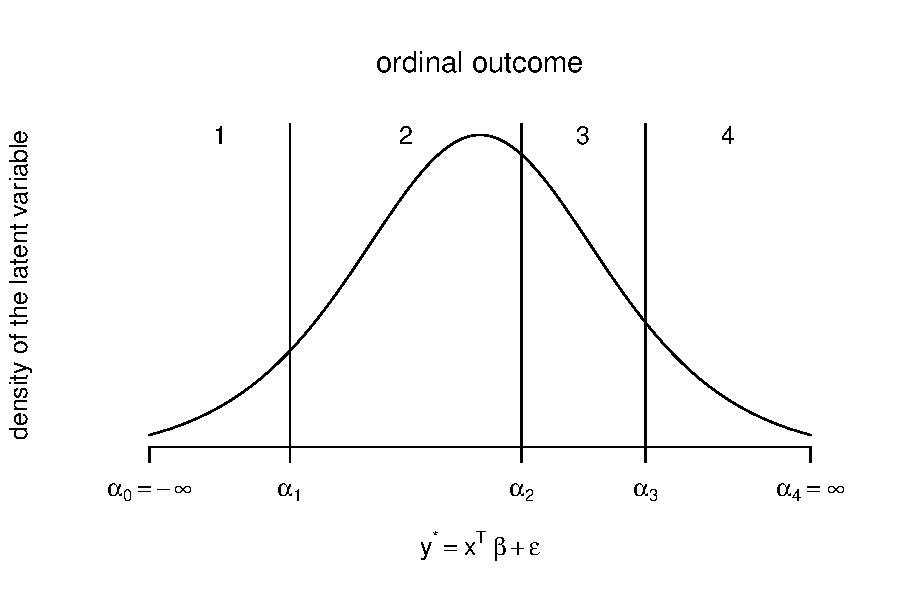
\includegraphics[width = 0.95\textwidth]{figures/ordinal_latent.pdf}
\caption{Latent variable representation of the ordinal outcome}
\label{fig::latent-ordinal}
\end{figure}



The unknown parameters are $(\beta,\alpha_{1},\ldots,\alpha_{K-1})$.
The distribution of the latent error term $g(\cdot)$ is known, for
example, it can be logistic or Normal. The former results in the proportional
odds logistic model, and the latter results in the ordered Probit
model. Based on the latent linear model, we can compute 
\begin{align*}
\pr(y_{i}  \leq k\mid x_{i}) &=\pr(y_{i}^{*}\leq\alpha_{k}\mid x_{i})\\
 & =\pr(x_{i}^{\T}\beta+\varepsilon_{i}\leq\alpha_{k}\mid x_{i})\\
 & =\pr(\varepsilon_{i}\leq\alpha_{k}-x_{i}^{\T}\beta\mid x_{i})\\
 & =g(\alpha_{k}-x_{i}^{\T}\beta).
\end{align*}
I will focus on the proportional odds logistic model in the main text and defer the details for the ordered Probit model to Problem \ref{hw18::ordered-probit}.
With this model, we have
\[
\pr(y_{i}\leq k\mid x_{i})=\frac{e^{\alpha_{k}-x_{i}^{\T}\beta}}{1+e^{\alpha_{k}-x_{i}^{\T}\beta}}
\]
or
\begin{equation}
\text{logit}\{  \pr(y_{i}\leq k\mid x_{i})  \} =\log\frac{\pr(y_{i}\leq k\mid x_{i})}{\pr(y_{i}>k\mid x_{i})}=\alpha_{k}-x_{i}^{\T}\beta . \label{eq:proportional-odds}
\end{equation}
The model has the ``proportional odds'' property because
$$
\frac{\pr(y_{i}\leq k\mid \ldots, x_{ij}+1,\ldots )}{\pr(y_{i}>k\mid \ldots, x_{ij}+1,\ldots)} 
\Big/ \frac{\pr(y_{i}\leq k\mid \ldots, x_{ij},\ldots)}{\pr(y_{i}>k\mid \ldots, x_{ij},\ldots)}
= e^{-\beta_j}
$$
which is a positive constant not depending on $k$. 


%We cannot change the right-hand side of (\ref{eq:proportional-odds}) to $\alpha_{k}-x_{i}^{\T}\beta_{k}$ because the general model cannot ensure (\ref{eq:ordering-information}). 
The sign of $x_{i}^{\T}\beta$ is negative due to the latent variable
representation. Some textbooks and software packages use a positive
sign, but the function \ri{polr} in package \ri{MASS} of \ri{R} uses (\ref{eq:proportional-odds}).


The proportional odds model implies a quite complicated form
of the probability for each category:
$$
\pr(y_{i}=k\mid x_{i})=\frac{e^{\alpha_{k}-x_{i}^{\T}\beta}}{1+e^{\alpha_{k}-x_{i}^{\T}\beta}}-\frac{e^{\alpha_{k-1}-x_{i}^{\T}\beta}}{1+e^{\alpha_{k-1}-x_{i}^{\T}\beta}}, \quad  (k=1,\ldots,K).
$$
%\[
%\begin{cases}
%\pr(y_{i}=1\mid x_{i})=\frac{e^{\alpha_{1}-x_{i}^{\T}\beta}}{1+e^{\alpha_{1}-x_{i}^{\T}\beta}},\\
%\pr(y_{i}=k\mid x_{i})=\frac{e^{\alpha_{k}-x_{i}^{\T}\beta}}{1+e^{\alpha_{k}-x_{i}^{\T}\beta}}-\frac{e^{\alpha_{k-1}-x_{i}^{\T}\beta}}{1+e^{\alpha_{k-1}-x_{i}^{\T}\beta}}, & (j=2,\ldots,J-1)\\
%\pr(y_{i}=K\mid x_{i})=1-\frac{e^{\alpha_{K-1}-x_{i}^{\T}\beta}}{1+e^{\alpha_{K-1}-x_{i}^{\T}\beta}}.
%\end{cases}
%\]
So the likelihood function is
\begin{eqnarray*}
L(\beta,\alpha_{1},\ldots,\alpha_{K-1}) 
&=& \prod_{i=1}^n \prod_{k=1}^K \{ \pr(y_{i}=k\mid x_{i})\}^{1(y_i = k)} \\
&=&  \prod_{i=1}^n \prod_{k=1}^K  \left( \frac{e^{\alpha_{k}-x_{i}^{\T}\beta}}{1+e^{\alpha_{k}-x_{i}^{\T}\beta}}-\frac{e^{\alpha_{k-1}-x_{i}^{\T}\beta}}{1+e^{\alpha_{k-1}-x_{i}^{\T}\beta}}\right)^{1(y_i = k)} .
\end{eqnarray*} 

The log-likelihood function is concave \citep{pratt1981concavity, burridge1981note}, and it is strictly concave in most cases. The function \ri{polr} in the \ri{R} package \ri{MASS} computes the MLE of the proportional odds model using the BFGS algorithm. It uses the explicit formulas of the gradient of the log-likelihood function, and computes the Hessian matrix numerically. I relegate the formulas of the gradient as a homework problem. For more details of the Hessian matrix, see \citet{agresti2010analysis}, which is a textbook discussion on modeling ordinal data. 
 
 


\section{A case study}\label{sec::multinomial-case-study}


I use a small observational dataset from the Karolinska Institute in Stockholm, Sweden to illustrate the application of logistic regressions. \citet{rubin2008objective} used this dataset to investigate whether it is better for cardia cancer patients to be treated in a large or small-volume hospital, where volume is defined by the number of patients with cardia cancer treated in recent years. I use the following variables: \ri{highdiag} indicating whether a patient was diagnosed at a high volume hospital, \ri{hightreat} indicating whether a patient was treated at a high volume hospital, \ri{age} representing the age, \ri{rural} indicating whether the patient was from a rural area, and \ri{survival} representing the years of survival after diagnosis with three categories (``1'', ``2-4'', ``5+''). The \ri{R} code is in \ri{code20.5.R}.

 
\begin{lstlisting}
karolinska = read.table("karolinska.txt", header = TRUE)
karolinska = karolinska[, c("highdiag", "hightreat",
                            "age", "rural", 
                            "male", "survival")]
\end{lstlisting}


\subsection{Binary logistic for the treatment}


We have two choices of the treatment: \ri{highdiag} and \ri{hightreat}. The logistic fit of \ri{highdiag} on covariates is shown below.

\begin{lstlisting}
> diagglm = glm(highdiag ~ age + rural + male, 
+               data = karolinska, 
+               family = binomial(link = "logit"))
> summary(diagglm)

Call:
glm(formula = highdiag ~ age + rural + male, family = binomial(link = "logit"), 
    data = karolinska)

Deviance Residuals: 
     Min        1Q    Median        3Q       Max  
-2.06147  -0.98645  -0.05759   1.01391   1.75696  

Coefficients:
            Estimate Std. Error z value Pr(>|z|)    
(Intercept)  3.46604    1.14545   3.026 0.002479 ** 
age         -0.03124    0.01481  -2.110 0.034854 *  
rural       -1.26322    0.34530  -3.658 0.000254 ***
male        -0.97524    0.41303  -2.361 0.018216 *  
\end{lstlisting}

The logistic fit of \ri{hightreat} is shown below.

\begin{lstlisting}
> treatglm = glm(hightreat ~ age + rural + male, 
+               data = karolinska, 
+               family = binomial(link = "logit"))
> summary(treatglm)

Call:
glm(formula = hightreat ~ age + rural + male, family = binomial(link = "logit"), 
    data = karolinska)

Deviance Residuals: 
    Min       1Q   Median       3Q      Max  
-2.2912  -0.9978   0.5387   0.8408   1.4810  

Coefficients:
            Estimate Std. Error z value Pr(>|z|)    
(Intercept)  6.44683    1.49544   4.311 1.63e-05 ***
age         -0.06297    0.01890  -3.332 0.000862 ***
rural       -1.28777    0.39572  -3.254 0.001137 ** 
male        -0.74856    0.45285  -1.653 0.098329 .  
\end{lstlisting}


Both treatments are associated with the covariates. \ri{hightreat} is more strongly associated with age.   \citet{rubin2008objective} argued that \ri{highdiag} is more random than  \ri{hightreat}, and may have weaker association with other hidden covariates. For each model below, I fit the data twice corresponding to two choices of treatment.  Overall, we should trust the results with \ri{highdiag} more based on \citet{rubin2008objective}'s argument. 

 

\subsection{Binary logistic for the outcome}


I first fit binary logistic models for the dichotomized outcome indicating whether the patient survived longer than a year after diagnosis. 

\begin{lstlisting}
> karolinska$loneyear = (karolinska$survival != "1")
> loneyearglm = glm(loneyear ~ highdiag + age + rural + male,
+                  data = karolinska, 
+                  family = binomial(link = "logit"))
> summary(loneyearglm)

Call:
glm(formula = loneyear ~ highdiag + age + rural + male, family = binomial(link = "logit"), 
    data = karolinska)

Deviance Residuals: 
    Min       1Q   Median       3Q      Max  
-1.1755  -0.9936  -0.7739   1.3024   1.8557  

Coefficients:
            Estimate Std. Error z value Pr(>|z|)  
(Intercept) -1.22919    1.15545  -1.064   0.2874  
highdiag     0.13684    0.36586   0.374   0.7084  
age         -0.00389    0.01411  -0.276   0.7829  
rural        0.33360    0.35798   0.932   0.3514  
male         0.86706    0.44034   1.969   0.0489 *
\end{lstlisting}

\ri{highdiag} is not significant in the above regression. 


\begin{lstlisting}
> loneyearglm = glm(loneyear ~ hightreat + age + rural + male, 
+                   data = karolinska, 
+                   family = binomial(link = "logit"))
> summary(loneyearglm)

Call:
glm(formula = loneyear ~ hightreat + age + rural + male, family = binomial(link = "logit"), 
    data = karolinska)

Deviance Residuals: 
    Min       1Q   Median       3Q      Max  
-1.3767  -0.9683  -0.6784   1.0813   2.0833  

Coefficients:
             Estimate Std. Error z value Pr(>|z|)   
(Intercept) -3.353977   1.317942  -2.545  0.01093 * 
hightreat    1.417458   0.455603   3.111  0.00186 **
age          0.008725   0.014840   0.588  0.55655   
rural        0.633278   0.368525   1.718  0.08572 . 
male         1.079973   0.452191   2.388  0.01693 * 
\end{lstlisting} 


\ri{hightreat} is significant in the above regression. 


\subsection{Multinomial logistic for the outcome}

I then fit multinomial logistic models for the outcome with three categories. 

\begin{lstlisting}
> library(nnet)
> yearmultinom = multinom(survival ~ highdiag + age + rural + male,
+                         data = karolinska)
# weights:  18 (10 variable)
initial  value 173.580742 
iter  10 value 134.331992
final  value 134.130815 
converged
> summary(yearmultinom)
Call:
multinom(formula = survival ~ highdiag + age + rural + male, 
    data = karolinska)

Coefficients:
    (Intercept)    highdiag          age     rural      male
2-4   -1.075818 -0.06973187 -0.004624030 0.1744256 0.5028786
5+    -4.180416  0.64036289 -0.001846453 0.7365111 2.1628717

Std. Errors:
    (Intercept)  highdiag        age     rural      male
2-4    1.286987 0.4113006 0.01596377 0.4014718 0.4716831
5+     2.003581 0.5816365 0.02148936 0.5741017 1.0741239

Residual Deviance: 268.2616 
AIC: 288.2616 
> predict(yearmultinom, type = "probs")[1:5, ]
          1       2-4         5+
1 0.5950631 0.2647047 0.14023222
2 0.5941802 0.2655369 0.14028293
3 0.8081376 0.1718963 0.01996613
4 0.5950631 0.2647047 0.14023222
5 0.6366929 0.2260086 0.13729849
\end{lstlisting}

\ri{highdiag} is not significant above.  The \ri{predict} function gives the fitted probabilities for all categories of the outcome. 

\begin{lstlisting}
> yearmultinom = multinom(survival ~ hightreat + age + rural + male,
+                         data = karolinska)
# weights:  18 (10 variable)
initial  value 173.580742 
iter  10 value 129.548642
final  value 129.283739 
converged
> summary(yearmultinom)
Call:
multinom(formula = survival ~ hightreat + age + rural + male, 
    data = karolinska)

Coefficients:
    (Intercept) hightreat         age     rural      male
2-4   -3.312433  1.326354 0.008527561 0.5186654 0.7514451
5+    -5.935172  1.627711 0.008978103 0.9063831 2.2780877

Std. Errors:
    (Intercept) hightreat        age     rural      male
2-4    1.463258 0.5141127 0.01660648 0.4085976 0.4806953
5+     2.190305 0.7320788 0.02244867 0.5645595 1.0739669

Residual Deviance: 258.5675 
AIC: 278.5675 
\end{lstlisting}

\ri{hightreat} is significant above. 





\subsection{Proportional odds logistic for the outcome}

 


The multinomial logisitic model does not reflect the ordering information of the outcome. For instance, in the regression with \ri{highdiag}, the coefficient for level ``2-4'' is  $-0.06973187<0$, but the coefficient for level ``5+'' is $0.64036289 >0$, which means that \ri{highdiag} decreases the probability of ``2-4'' but increases the probability of ``5''. However, this is illogical since a patient must first live longer than two years and then live longer than five years. Nevertheless, it is not a severe problem in this case study because those coefficients are not significant. 


\begin{lstlisting}
> library(MASS)
> yearpo = polr(survival ~ highdiag + age + rural + male, 
+               Hess = TRUE, 
+               data = karolinska)
> summary(yearpo)
Call:
polr(formula = survival ~ highdiag + age + rural + male, data = karolinska, 
    Hess = TRUE)

Coefficients:
             Value Std. Error t value
highdiag  0.216755    0.35892  0.6039
age      -0.002881    0.01378 -0.2091
rural     0.371898    0.35313  1.0532
male      0.943955    0.43588  2.1656

Intercepts:
       Value   Std. Error t value
1|2-4   1.4079  1.1309     1.2450
2-4|5+  2.9284  1.1514     2.5434

Residual Deviance: 271.0778 
AIC: 283.0778 
> predict(yearpo, type = "probs")[1:5, ]
          1       2-4         5+
1 0.5862465 0.2800892 0.13366427
2 0.5855475 0.2804542 0.13399823
3 0.8087341 0.1421065 0.04915948
4 0.5862465 0.2800892 0.13366427
5 0.6205983 0.2615112 0.11789050
\end{lstlisting}

\ri{highdiag} is not significant above. The \ri{predict} function gives the fitted probabilities of three categories. 


\begin{lstlisting}
> yearpo = polr(survival ~ hightreat + age + rural + male, 
+               Hess = TRUE, 
+               data = karolinska)
> summary(yearpo)
Call:
polr(formula = survival ~ hightreat + age + rural + male, data = karolinska, 
    Hess = TRUE)

Coefficients:
             Value Std. Error t value
hightreat 1.399538    0.44518  3.1438
age       0.008032    0.01438  0.5584
rural     0.638862    0.35450  1.8022
male      1.122698    0.44377  2.5299

Intercepts:
       Value  Std. Error t value
1|2-4  3.3273 1.2752     2.6092 
2-4|5+ 4.9258 1.3106     3.7583 

Residual Deviance: 260.2831 
AIC: 272.2831 
\end{lstlisting}

\ri{hightreat} is significant above. 



\section{Discrete choice models}\label{sec::discretechioce}


\subsection{Model}
The covariates in model \eqref{eq::multinomial-logistic} depend only on individuals. 
\citet{mcfadden1974conditional} extends it to allow for choice-specific covariates $z_{ik}$. His formulation is based on the latent utility representation: 
\[
\begin{cases}
U_{i1} & =   z_{i1}^{\T} \theta +\varepsilon_{i1},\\
\vdots\\
U_{iK} & =z_{iK}^{\T} \theta +\varepsilon_{iK},
\end{cases}
\]
where $\varepsilon_{i1},\ldots,\varepsilon_{iK}$ are IID standard Gumbel. Unit $i$ chooses $k$ if $k$ has the highest utility. Lemma \ref{lemma::mcfadden} implies that
\begin{eqnarray}
\pi_{k}(z_{i})=\pi_{k}(z_{i},\theta)=\frac{e^{  z_{ik}^{\T}\theta }  }{\sum_{ l =1}^{K}e^{ z_{i l }^{\T}\theta } } ,\qquad(k=1,\ldots,K) .
\label{eq::multinomial-logistic-mcfadden}
\end{eqnarray}


Model \eqref{eq::multinomial-logistic-mcfadden} seems rather similar to model \eqref{eq::multinomial-logistic}. However, there are many subtle differences. First, a component of $z_{ik}$ may vary only with choice $k$, for example, it can represent the price of choice $k$. Partition $z_{ik}$ into three types of covariates: $x_i$ that only vary cross individuals, $c_k$ that only vary across choices, and $w_{ik}$ that vary across both individuals and choices. Model \eqref{eq::multinomial-logistic-mcfadden} reduces to
$$
\pi_{k}(z_{i})  =\frac{e^{  x_{i}^{\T}\theta_x + c_k^{\T}\theta_c + w_{ik}^{\T} \theta_w }  }
{\sum_{ l =1}^{K}e^{ x_{i}^{\T}\theta_x + c_{ l }^{\T}\theta_c + w_{i l }^{\T} \theta_w }  }  
=\frac{e^{   c_k^{\T}\theta_c + w_{ik}^{\T} \theta_w }  }
{\sum_{ l =1}^{K}e^{   c_{ l }^{\T}\theta_c + w_{i l }^{\T} \theta_w } }  ,
$$
that is, the individual-specific covariates drop out. Therefore, $z_{ik}$ in model \eqref{eq::multinomial-logistic-mcfadden} does not contain covariates that vary only with individuals. In particular, $z_{ik}$ in model \eqref{eq::multinomial-logistic-mcfadden} does not contain the constant, but in contrast, the $x_i$ in model \eqref{eq::multinomial-logistic} ususally contains the intercept by default. 

Second, if we want to use individual-specific covariates in the model, they must have choice-specific coefficients. So a more general model unifying \eqref{eq::multinomial-logistic} and \eqref{eq::multinomial-logistic-mcfadden} is
\begin{eqnarray}
%\pi_{k}(z_{i})=
\pi_{k}(x_{i}, w_{ik}, \theta, \beta)=\frac{e^{  w_{ik}^{\T}\theta + x_i^{\T} \beta_k }  }{\sum_{ l =1}^{K}e^{ w_{i l }^{\T}\theta + x_i^{\T} \beta_{ l } }},\qquad(k=1,\ldots,K) .
\label{eq::multinomial-logistic-unify}
\end{eqnarray}
Equivalently, we can create pseudo covariates $z_{ik}$ as the original $w_{ik}$ together with interaction of $x_i$ and the dummy for choice $k$. For example, if $K = 3$ and $x_i$ contain the intercept and a scalar individual-specific covariate, then $(z_{i1}, z_{i2}, z_{i3})$ are
\begin{eqnarray*}
\begin{pmatrix}
z_{i1} \\
z_{i2} \\
z_{i3}
\end{pmatrix}
= 
\begin{pmatrix}
w_{i1} & 1 & 0 & x_i & 0 \\
w_{i2} & 0 & 1 & 0 & x_i \\
w_{i3} & 0 & 0 & 0 & 0
\end{pmatrix},
\end{eqnarray*}
where $K=3$ is the reference level. 
So with augmented covariates, the discrete choice model \eqref{eq::multinomial-logistic-mcfadden} is strictly more general than the multinomial logistic model \eqref{eq::multinomial-logistic}. In the special case with $K=2$, model \eqref{eq::multinomial-logistic-mcfadden} reduces to
$$
\pr(y_i = 1\mid   x_i ) = \frac{  e^{  x_i^{\T} \beta }   }{   1 + e^{  x_i^{\T} \beta }  }
$$
where $x_i = z_{i1} - z_{i2}$. 




Based on the model specification \eqref{eq::multinomial-logistic-mcfadden}, the log likelihood function is
$$
\log L(\theta) 
%= \sumn \sum_{k=1}^K 1(y_i = k) \log \frac{e^{  z_{ik}^{\T}\theta }  }{\sum_{ l =1}^{K}e^{ z_{i l }^{\T}\theta } }
= \sumn \sum_{k=1}^K 1(y_i = k)  \left(  z_{ik}^{\T}\theta -   \log \sum_{ l =1}^{K}e^{ z_{i l }^{\T}\theta }   \right).
$$
So the score function is
\begin{eqnarray*}
\frac{\partial }{ \partial \theta } \log L(\theta) 
&=& \sumn \sum_{k=1}^K 1(y_i = k)    \left(  z_{ik}  -   
\frac{   \sum_{ l =1}^{K}e^{ z_{i l }^{\T}\theta }  z_{i l } }{\sum_{ l =1}^{K}e^{ z_{i l }^{\T}\theta }  } \right) \\
&=& \sumn \sum_{k=1}^K 1(y_i = k)    \{  z_{ik}  -  E(z_{ik};\theta)    \},
\end{eqnarray*}
where $E(\cdot; \theta) $ is the average value of $\{ z_{i1}, \ldots, z_{iK} \}$ over the probability mass function
$$
p_k(\theta) = e^{z_{ik}^{\T}\theta} / \sum_{ l =1}^{K}e^{ z_{i l }^{\T}\theta }.
$$
The Hessian matrix is
\begin{eqnarray*}
&&\frac{\partial^2 }{ \partial \theta\partial \theta^{\T}  } \log L(\theta)  \\
&=& - \sumn \sum_{k=1}^K 1(y_i = k)  
\frac{   \sum_{ l =1}^{K}e^{ z_{i l }^{\T}\theta }  z_{i l } z_{i l }^{\T}\sum_{ l =1}^{K}e^{ z_{i l }^{\T}\theta }
- \sum_{ l =1}^{K}e^{ z_{i l }^{\T}\theta }  z_{i l } \sum_{ l =1}^{K}e^{ z_{i l }^{\T}\theta }  z_{i l }^{\T}
 }{  (\sum_{ l =1}^{K}e^{ z_{i l }^{\T}\theta })^2  }  \\
 &=& - \sumn \sum_{k=1}^K 1(y_i = k)   \cov(z_{ik}; \theta),
\end{eqnarray*}
where $\cov(\cdot; \theta) $ is the covariance matrix of $\{ z_{i1}, \ldots, z_{iK} \}$ over the probability mass function defined above. 
From these formulas, we can easily compute the MLE using Newton's method and obtain its asymptotic distribution based on the inverse of the Fisher information matrix. 

\subsection{Example}

The \ri{R} package \ri{mlogit} provides a function \ri{mlogit} to fit the general discrete logistic model \citep{croissant2020estimation}. 
Here I use an example from this package to illustrate the model fitting of \ri{mlogit}. The \ri{R} code is in \ri{code20.6.R}.
\begin{lstlisting}
> library("nnet")
> library("mlogit")
> data("Fishing")
> head(Fishing)
     mode price.beach price.pier price.boat price.charter
1 charter     157.930    157.930    157.930       182.930
2 charter      15.114     15.114     10.534        34.534
3    boat     161.874    161.874     24.334        59.334
4    pier      15.134     15.134     55.930        84.930
5    boat     106.930    106.930     41.514        71.014
6 charter     192.474    192.474     28.934        63.934
  catch.beach catch.pier catch.boat catch.charter   income
1      0.0678     0.0503     0.2601        0.5391 7083.332
2      0.1049     0.0451     0.1574        0.4671 1250.000
3      0.5333     0.4522     0.2413        1.0266 3750.000
4      0.0678     0.0789     0.1643        0.5391 2083.333
5      0.0678     0.0503     0.1082        0.3240 4583.332
6      0.5333     0.4522     0.1665        0.3975 4583.332
\end{lstlisting}

The dataset \ri{Fishing} is in the ``wide'' format, where \ri{mode} denotes the choice of four modes of fishing (beach, pier, boat and charter), \ri{price} and \ri{catch} denote the price and catching rates which are choice-specific, \ri{income} is individual-specific. 
We need to first transform the dataset into ``long'' format.

\begin{lstlisting}
> Fish  = dfidx(Fishing, 
+               varying = 2:9, 
+               shape = "wide", 
+               choice = "mode")
> head(Fish)
~~~~~~~
 first 10 observations out of 4728 
~~~~~~~
    mode   income   price  catch    idx
1  FALSE 7083.332 157.930 0.0678 1:each
2  FALSE 7083.332 157.930 0.2601 1:boat
3   TRUE 7083.332 182.930 0.5391 1:rter
4  FALSE 7083.332 157.930 0.0503 1:pier
5  FALSE 1250.000  15.114 0.1049 2:each
6  FALSE 1250.000  10.534 0.1574 2:boat
7   TRUE 1250.000  34.534 0.4671 2:rter
8  FALSE 1250.000  15.114 0.0451 2:pier
9  FALSE 3750.000 161.874 0.5333 3:each
10  TRUE 3750.000  24.334 0.2413 3:boat
\end{lstlisting}

Using only choice-specific covariates, we have the following fitted model:

\begin{lstlisting}
> summary(mlogit(mode ~ 0 + price + catch, data = Fish))

Call:
mlogit(formula = mode ~ 0 + price + catch, data = Fish, method = "nr")

Frequencies of alternatives:choice
  beach    boat charter    pier 
0.11337 0.35364 0.38240 0.15059 

nr method
6 iterations, 0h:0m:0s 
g'(-H)^-1g = 0.000179 
successive function values within tolerance limits 

Coefficients :
        Estimate Std. Error z-value  Pr(>|z|)    
price -0.0204765  0.0012231 -16.742 < 2.2e-16 ***
catch  0.9530982  0.0894134  10.659 < 2.2e-16 ***

Log-Likelihood: -1312
\end{lstlisting}

If we do not enforce \ri{0 + price}, we allow for intercepts that vary across choices:

\begin{lstlisting}
> summary(mlogit(mode ~ price + catch, data = Fish))

Call:
mlogit(formula = mode ~ price + catch, data = Fish, method = "nr")

Frequencies of alternatives:choice
  beach    boat charter    pier 
0.11337 0.35364 0.38240 0.15059 

nr method
7 iterations, 0h:0m:0s 
g'(-H)^-1g = 6.22E-06 
successive function values within tolerance limits 

Coefficients :
                      Estimate Std. Error  z-value  Pr(>|z|)    
(Intercept):boat     0.8713749  0.1140428   7.6408 2.154e-14 ***
(Intercept):charter  1.4988884  0.1329328  11.2755 < 2.2e-16 ***
(Intercept):pier     0.3070552  0.1145738   2.6800 0.0073627 ** 
price               -0.0247896  0.0017044 -14.5444 < 2.2e-16 ***
catch                0.3771689  0.1099707   3.4297 0.0006042 ***

Log-Likelihood: -1230.8
McFadden R^2:  0.17823 
Likelihood ratio test : chisq = 533.88 (p.value = < 2.22e-16)
\end{lstlisting}

Using only individual-specific covariates, we have the following fitted model:

\begin{lstlisting}
> summary(mlogit(mode ~ 0 | income, data = Fish))

Call:
mlogit(formula = mode ~ 0 | income, data = Fish, method = "nr")

Frequencies of alternatives:choice
  beach    boat charter    pier 
0.11337 0.35364 0.38240 0.15059 

nr method
4 iterations, 0h:0m:0s 
g'(-H)^-1g = 8.32E-07 
gradient close to zero 

Coefficients :
                       Estimate  Std. Error z-value  Pr(>|z|)    
(Intercept):boat     7.3892e-01  1.9673e-01  3.7560 0.0001727 ***
(Intercept):charter  1.3413e+00  1.9452e-01  6.8955 5.367e-12 ***
(Intercept):pier     8.1415e-01  2.2863e-01  3.5610 0.0003695 ***
income:boat          9.1906e-05  4.0664e-05  2.2602 0.0238116 *  
income:charter      -3.1640e-05  4.1846e-05 -0.7561 0.4495908    
income:pier         -1.4340e-04  5.3288e-05 -2.6911 0.0071223 ** 

Log-Likelihood: -1477.2
McFadden R^2:  0.013736 
Likelihood ratio test : chisq = 41.145 (p.value = 6.0931e-09)
\end{lstlisting}

It is equivalent to fitting the multinomial logistic model:

\begin{lstlisting}
summary(multinom(mode ~ income, data = Fishing))
\end{lstlisting}

The most general model includes all covariates.

\begin{lstlisting}
> summary(mlogit(mode ~ price + catch | income, data = Fish))

Call:
mlogit(formula = mode ~ price + catch | income, data = Fish, 
    method = "nr")

Frequencies of alternatives:choice
  beach    boat charter    pier 
0.11337 0.35364 0.38240 0.15059 

nr method
7 iterations, 0h:0m:0s 
g'(-H)^-1g = 1.37E-05 
successive function values within tolerance limits 

Coefficients :
                       Estimate  Std. Error  z-value  Pr(>|z|)
(Intercept):boat     5.2728e-01  2.2279e-01   2.3667 0.0179485
(Intercept):charter  1.6944e+00  2.2405e-01   7.5624 3.952e-14
(Intercept):pier     7.7796e-01  2.2049e-01   3.5283 0.0004183
price               -2.5117e-02  1.7317e-03 -14.5042 < 2.2e-16
catch                3.5778e-01  1.0977e-01   3.2593 0.0011170
income:boat          8.9440e-05  5.0067e-05   1.7864 0.0740345
income:charter      -3.3292e-05  5.0341e-05  -0.6613 0.5084031
income:pier         -1.2758e-04  5.0640e-05  -2.5193 0.0117582
                       
(Intercept):boat    *  
(Intercept):charter ***
(Intercept):pier    ***
price               ***
catch               ** 
income:boat         .  
income:charter         
income:pier         *  

Log-Likelihood: -1215.1
McFadden R^2:  0.18868 
Likelihood ratio test : chisq = 565.17 (p.value = < 2.22e-16)
\end{lstlisting}


\subsection{More comments}


The assumption of Gumbel error terms is very strong. However, relaxing this assumption leads to much more complicated forms of the conditional probabilities of the outcome. The model \eqref{eq::multinomial-logistic-mcfadden} implies that 
$$
\frac{  \pi_k(z_i) }{ \pi_l(z_i) } = \exp\{  (z_{ik} - z_{il})^{\T} \theta   \},
$$
so the choice between $k$ and $l$ does not depend on the existence of other choices. This is called the
independence of irrelevant alternatives (IIA) assumption. This is often a plausible assumption. However, it may be violated. For example, with the apple and orange, someone chooses the apple; but with the apple, orange, and banana, s/he may choose the orange.

The model \eqref{eq::multinomial-logistic-mcfadden}  is the basic form of the discrete choice model. \citet{train2009discrete} is a monograph on this topic which provides many extensions.
%\footnote{Daniel McFadden shared the 2000 Nobel Memorial Prize in Economic Sciences with James Heckman ``for his development of theory and methods for analyzing discrete choice.''}. 


\section{Homework problems}


\paragraph{Inverse model for the  multinomial logit model}\label{hw18::inverse-multinom}


The following result extends Theorem \ref{thm::inverse-logit}. 

Assume that 
\begin{eqnarray}
y_{i}\sim\text{Multinomial}(1; q_1, \ldots, q_K),
\label{eq::y-marginal}
\end{eqnarray}
and
\begin{eqnarray}
x_{i}\mid y_{i}=k\sim\N(\mu_{k},\Sigma),
\label{eq::xgiveny}
\end{eqnarray} 
where $x_i$ does not contain $1$.
We can verify that $y_{i}\mid x_{i}$ follows a multinomial logit model as shown in the theorem below.  


\begin{theorem}
\label{thm::inverse-multinom-logit}
Under \eqref{eq::y-marginal} and \eqref{eq::xgiveny}, we have
$$
 \pr(y_i =k\mid x_i)   =   \frac{  e^{\alpha_k + x_i^{\T} \beta_k} }{   \sum_{l=1}^K e^{\alpha_l + x_i^{\T} \beta_l} } ,
$$
where
\begin{eqnarray*}
\label{eq::alpha-beta-lda}
\alpha_k = \log q_k -\frac{1}{2} \mu_k^{\T}\Sigma^{-1}\mu_k  ,\quad
\beta_k = \Sigma^{-1} \mu_k.
\end{eqnarray*}
\end{theorem}


Prove Theorem \ref{thm::inverse-multinom-logit}. 

 

\paragraph{Hessian matrix in the multinomial logit model}\label{hw18::hessian-multinom}

Prove that the Hessian matrix \eqref{eq::hessian-logit-categorical} of the log-likelihood function of the multinomial logit model is negative semi-definite. 


Hint: Use Proposition \ref{proposition:positive-semi-definite-multinomial}. 

\paragraph{Iteratively reweighted least squares algorithm for the multinomial logit model}\label{hw18::irls-multinom}

Similar to the binary logistic model, Newton's method for computing the MLE for the multinomial logit model can be written as iteratively reweighted least squares. Give the details. 

\paragraph{Score function of the proportional odds model}

Derive the explicit formulas of the score function of the proportional odds model. 


\paragraph{Ordered Probit regression}\label{hw18::ordered-probit}

If we choose $\varepsilon_i \mid x_i \sim \N(0,1)$ in \eqref{eq::latent-ordinal}, then the corresponding model is called the ordered Probit regression. Write down the likelihood function and derive the score function for this model. 

Remark: You can use the function \ri{polr} in \ri{R} to fit this model with the specification \ri{method = "probit"}. 

\paragraph{Case-control study and multinomial logistic model}\label{hw18::case-control-multinom}

This problem extends Theorem \ref{thm::case-control}. 

Assume that
$$
\pr(y_i = k\mid x_i) = \frac{  e^{\alpha_k + x_i^{\T} \beta_k} }{ \sum_{ l =1}^K e^{\alpha_{ l  }+ x_i^{\T} \beta_{ l }} }
$$
%with $\alpha_K=0$ and $\beta_K = 0$, and
and 
$$
\pr(s_i =1\mid y_i = k, x_i) = \pr(s_i =1\mid y_i = k ) = p_k 
$$
for $k=1,\ldots, K$. 
Show that 
$$
\pr(y_i = k\mid x_i, s_i = 1) = \frac{  e^{\tilde \alpha_k  + x_i^{\T} \beta_k} }{ \sum_{ l =1}^K e^{\tilde \alpha_{ l  }   + x_i^{\T} \beta_{ l }} }
$$
with $\tilde \alpha_k = \alpha_k + \log p_k$ for $k=1,\ldots, K$. 
 

 
